\documentclass[10pt]{article}
\usepackage[a4paper,margin=18mm]{geometry}
\usepackage{graphicx}
\usepackage{amsmath}
\usepackage{xcolor}
\usepackage{caption}
\usepackage[hidelinks]{hyperref}

\title{Causal Neuromuscular State-Conditioned Attention Pipeline}
\author{}
\date{}

\begin{document}
\maketitle

\begin{figure*}[ht]
  \centering
  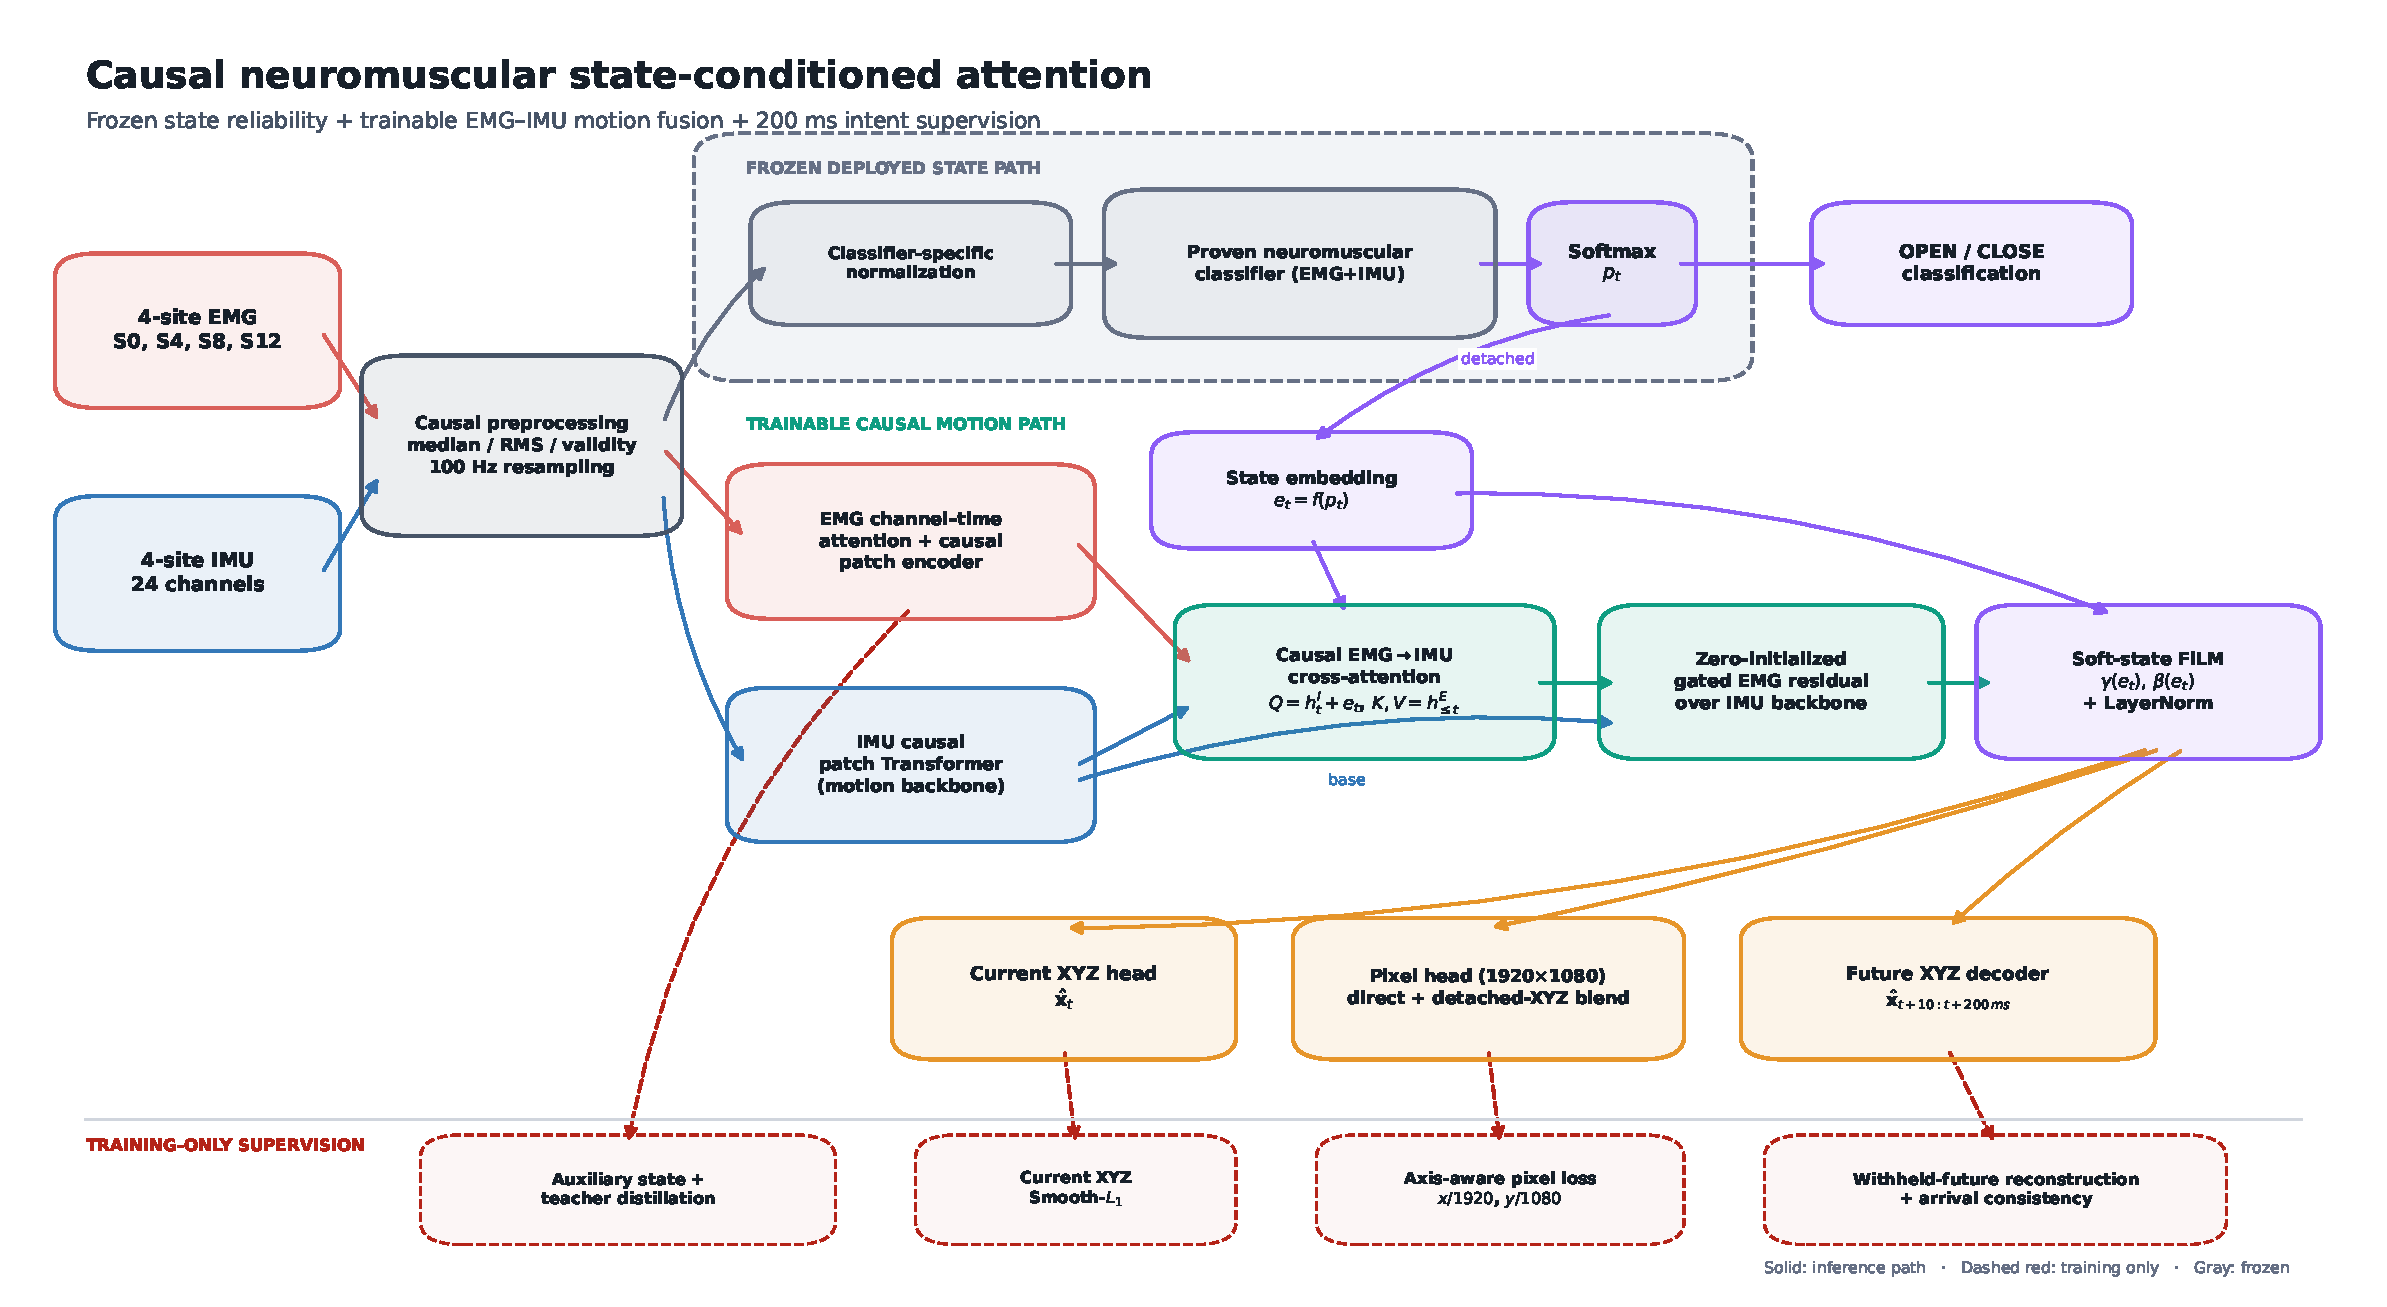
\includegraphics[width=\textwidth]{figures/neuro_classifier_state_attention_pipeline.pdf}
  \caption{%
  Proposed causal EMG--IMU pipeline. A previously validated neuromuscular
  classifier is frozen and evaluated using its original normalization. Its
  soft open/close probability $p_t$ is both the deployed gripper-state output
  and a detached conditioning signal for the trainable motion pathway. The
  EMG pathway performs channel--time selection, while the IMU pathway provides
  the motion backbone. Causal cross-attention uses the state-conditioned IMU
  feature as query and the EMG history as keys and values. A zero-initialized
  gated residual prevents unreliable EMG features from initially perturbing
  the IMU representation. Soft-state FiLM modulation produces the shared
  representation used for current position, screen position, and short-horizon
  future position. Future reconstruction and consistency terms are used only
  during training; no future wearable or VIVE sample is available at inference.}
  \label{fig:neuro-state-attention}
\end{figure*}

For a causal time index $t$, the fusion stage can be summarized as
\begin{align}
  p_t &= \operatorname{softmax}\!\left(C_{\mathrm{frozen}}
       (E_{\leq t},I_{\leq t})\right),\\
  a_t &= \operatorname{MHA}\!\left(
       Q=h_t^I+f(p_t),\;K=h_{\leq t}^E,\;V=h_{\leq t}^E\right),\\
  \widetilde h_t &= h_t^I+\sigma(g)R(a_t),\\
  z_t &= \operatorname{LN}\!\left(
       \widetilde h_t\odot[1+\gamma(f(p_t))]+\beta(f(p_t))\right).
\end{align}
Here $E$ and $I$ denote the preprocessed EMG and IMU streams, respectively;
$C_{\mathrm{frozen}}$ is not updated during motion-model training; and $R$ is
initialized to zero. The task heads predict current metric position
$\widehat{\mathbf{x}}_t$, normalized screen coordinates
$\widehat{\mathbf{u}}_t$, and future positions
$\widehat{\mathbf{x}}_{t+\tau}$ for $\tau\in\{10,\ldots,200\}$~ms. Screen
coordinates are converted independently as
\begin{equation}
  (\widehat x_{\mathrm{px}},\widehat y_{\mathrm{px}})
  =(1920\widehat u_x,\;1080\widehat u_y).
\end{equation}

\end{document}
